\documentclass{article}
\usepackage{graphicx} % Required for inserting images
\usepackage{pgfplots}
\pgfplotsset{compat = newest}
\usetikzlibrary{positioning, arrows.meta}
\usepgfplotslibrary{fillbetween}
\usepackage{amsmath}

\documentclass[12pt]{article}
\linespread{1.25}
\usepackage{times}

\usepackage{pgfplots}
\pgfplotsset{compat = newest}
\usetikzlibrary{positioning, arrows.meta}
\usepgfplotslibrary{fillbetween}
\usepackage{amsmath}
\title{AP Macroeconomics Models}
\author{Indivara K}

\date{December 2023}


\begin{document}


\maketitle

\textbf{**NOTE: The reader is assumed to understand basic economic terminology such as shifts, movements, models, and more. This is just a comprehensive review of the models tested on the AP Macro Exam.  Also remember that shocks only happen when exogenous determinants changes. Shocks cause shifts, cause variable to change.}










\newpage

\section{Supply and Demand (Market)}:

\textbf{Model:}
\begin{center}
\begin{tikzpicture}
\begin{axis}[
scale = 1.2,
xmin = 0, xmax = 10,
ymin = 0, ymax = 10,
axis lines* = left,
xtick = {0}, ytick = \empty,
clip = false,
]
% Supply and demand curves
\addplot[color = blue, very thick] coordinates {(1, 9) (9, 1)};
\addplot[color = red, very thick] coordinates {(1, 1) (9, 9)};
% Dashed lines
\addplot[color = black, dashed, thick] coordinates {(0, 5) (5, 5)
(5, 0)};
% Coordinate points
\addplot[color = black, mark = *, only marks, mark size = 3pt]
coordinates {(5, 5)};
% Labels
\node [right] at (current axis.right of origin) {\textit{Quantity of Good}, $Q$};
\node [above] at (current axis.above origin) {Price, $P$};
\node [above] at (5, 5.2) {$E$};
\node [left] at (0, 5) {$P_E$};
\node [below] at (5, 0) {$Q_E$};
\node [right] at (9, 1) {$D_0$};
\node [right] at (9, 9) {$S_0$};
\end{axis}
\end{tikzpicture}
\end{center}

\textbf{Determinants of Demand}:
Demand, otherwise known as consumer preference for that good, has factors exogenous to the Market that shift it.

\begin{enumerate}
    \item \textbf{Consumer Income}: The more money consumers make the more they will buy more of the good at every price point, representing a shift
    \item \textbf{Consumer Taste/Preference for the good}: When consumers have more liking for a good, they will buy more of it at every price point
    \item \textbf{Prices of Substitutes}: When a "rival" good's price changes it has a negative correlation with the demand for this current good. 
    \item \textbf{Prices of Complements}: When the price of a "grouping" of goods changes, it has a positive correlation with the demand for this good
    \item \textbf{Number of Consumers}: More consumers = more demand
    \item \textbf{Consumer Expecations of Price:} When consumers expect the price to increase, they will buy more now
\end{enumerate}



\textbf{Determinants of Supply}:
\begin{enumerate}
    \item \textbf{Costs of Production}: When a good costs more to produce, the supply of it will decrease
    \item \textbf{Improvement in Technology}: As the production technology improves, supply will increase
    \item \textbf{Prices of Substitutes in Production}: An increase in the price of substitute goods decreases the supply of the current good
    \item \textbf{Production regulations}: An increase in regulations leads to a decrease in supply
    \item  \textbf{Changes in taxes/subsidies}: Increase in taxes = decrease and supply; increase in subsidies = increase in supply
    \item \textbf{Number of Suppliers}: More suppliers = more supply
    \item \textbf{Supplier Expecations of Price:} When suppliers expect the price to increase, they will supply less now.

\end{enumerate}

\newpage










\section{Production Possibilities Frontier (PPC or PPF):}

\textbf{Model:}
\begin{center}
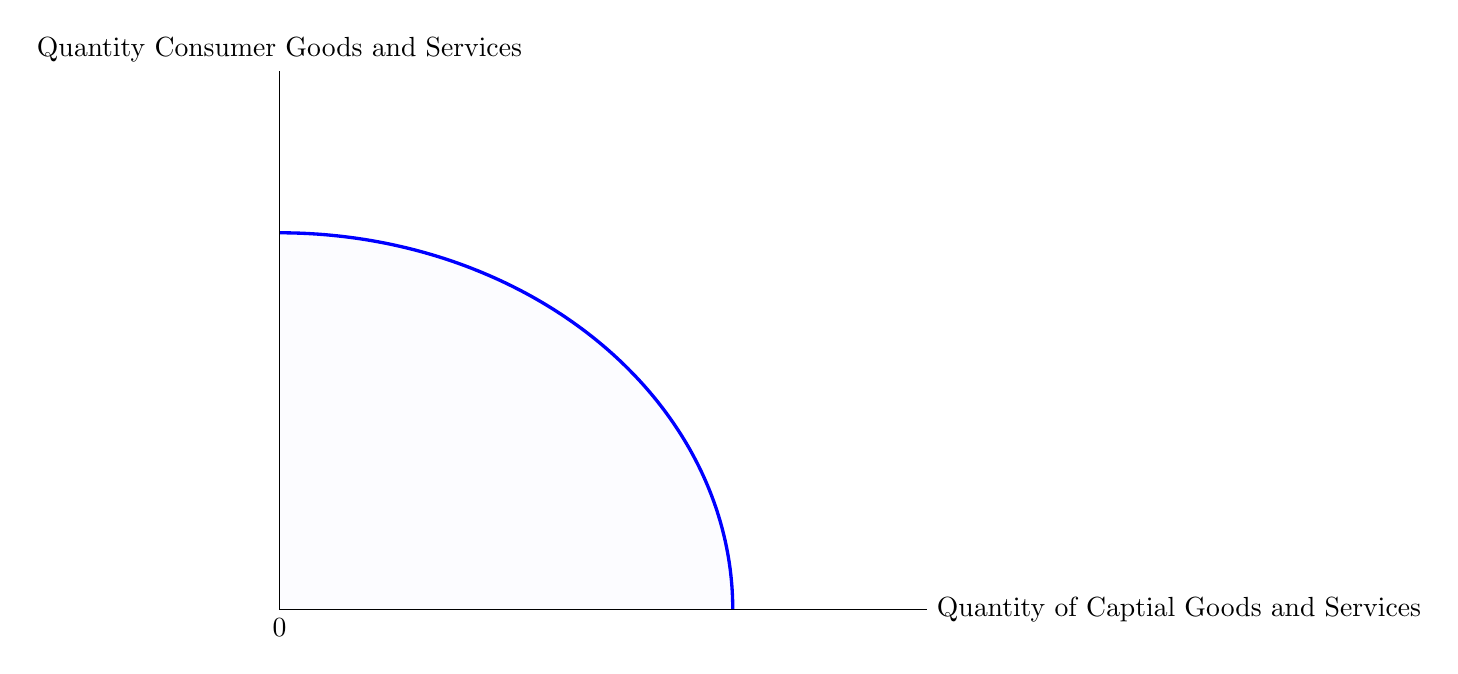
\begin{tikzpicture}
\begin{axis}[
scale = 1.2,
xmin = 0, xmax = 10,
ymin = 0, ymax = 10,
axis lines* = left,
xtick = {0}, ytick = \empty,
axis on top,
clip = false,
]
% Production-possibility frontier
\addplot [domain = 0:10, restrict y to domain = 0:10, samples=10000, color = blue, very thick, name path = frontier]{(49-x^2)^0.5};
\addplot [domain = 0:10, restrict y to domain = 0:10, draw = none, name path = axis]{0};

% Colouring areas
\addplot [blue,  opacity = 0.01] fill between [of = frontier and axis];

% Labels
\node [right] at (current axis.right of origin) {Quantity of Captial Goods and Services};
\node [above] at (current axis.above origin) {Quantity Consumer Goods and Services};
\end{axis}
\end{tikzpicture}
\end{center}
\textbf{Things to know about the PPC}:
\begin{enumerate}
    \item It follows the Law of Increasing Opportunity Costs, where the benefit of each additional good decreases
    \item The PPC is also used to determine allocative efficiency and terms of trade between two countries or individuals. This is based on the opportunity costs of production for each country.
    \item Points on the PPC are at maximum efficiency,
    \item Points inside the PPC are not (recession)
    \item  Points outside of the PPC are not feasible without any economic growth
    \begin{enumerate}
        \item Economic growth is caused by:
        \begin{enumerate}
            \item Increases in resources (land, labour, capital, and entrepreneurial ability)
            \item Productivity, which is increases in Human, Physical, and Technological capital
        \end{enumerate}
    \end{enumerate}
\end{enumerate}


\section{Aggregate Production Function:}

\textbf{Model:}
\begin{tikzpicture}
\begin{axis}[
  axis lines=middle,
  clip=false,
  ymin=0,
  xticklabels=\empty,
  yticklabels=\empty,
  legend pos=north west
]
\addplot+[mark=none,samples=200,unbounded coords=jump] {sqrt(x)};

\draw[fill] (axis cs:4,0) circle [radius=0.0pt] node[below right] {Quantity Physical Capital per Worker};
\draw[fill] (axis cs:{0,2}) circle [radius=0.0pt] node[above left] {Real GDP per Capita};
\end{axis}
\end{tikzpicture}
We can see the Law of Dimishing returns here, as the function increases by a decreasing amount with each extra increase in physical capital per worker.
\textbf{Causes of Shifts:}
Changes to quality of human capital, and technological capital will shift the curve. For example better education and productional technology will shift it upwards.  
\newpage()
\section{The Business Cycle}
\textbf{Model:}
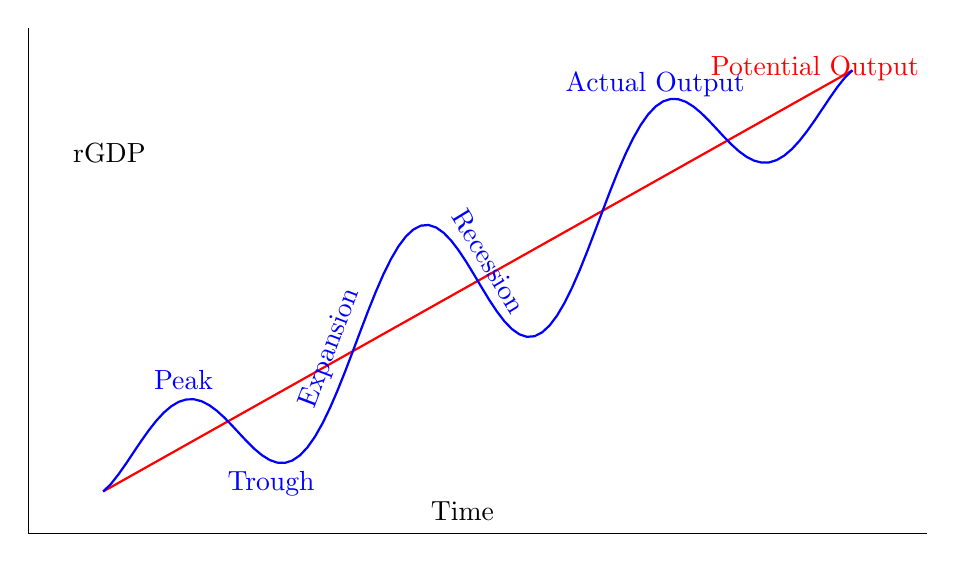
\begin{tikzpicture}
\begin{axis}[
    domain=0:6*pi,
    samples=100,
    axis lines*=left,
    xtick=\empty, ytick=\empty,
    width=13cm, height=8cm
]
\draw[fill] (axis cs:8,0) circle [radius=0.0pt] node[below right] {Time};

\draw[fill] (axis cs:-1,16) circle [radius=0.0pt] node[below right] {rGDP};
\addplot [thick, red] {x}
    node[pos = .95, anchor=south]{Potential Output}
;
\addplot [thick, blue] {x + 4*sin(deg(x)) * sin(deg(x/6))^0.5}
    node [pos=0.1, anchor=south] {Peak}
    node [pos=0.18, anchor=north] {Trough}
    node [pos=0.3, anchor=south, sloped] {Expansion}
    node [pos=0.49, anchor=south, sloped] {Recession}
    node[pos=.8, anchor=south] {Actual Output}
;
\end{axis}
\end{tikzpicture}
\textbf{Important Connections}:
\begin{enumerate}
    \item \textbf{The Business Cycle follows these two cycles}:
    \begin{enumerate}
        \item Bust Cycle (Actual $<$ Potential):
        \begin{enumerate}
            \item Consumer Confidence decreases
            \item Less spending
            \item More inventory
            \item Lowering Price Level
            \item Less revenue from businesses leads to firing
        \end{enumerate}
        \item Boom Cycle (Actual $>$ Potential):
        \begin{enumerate}
            \item Consumer and Business Confidence Increases
            \item More spending
            \item Less inventories
            \item Increase in the price level
            \item More revenue leads to hiring














\newpage
\section{AD/AS Model}
\textbf{Model:}
\begin{center}
\begin{tikzpicture}
\begin{axis}[
scale = 1.2,
xmin = 0, xmax = 10,
ymin = 0, ymax = 10,
axis lines* = left,
xtick = {0}, ytick = \empty,
clip = false,
]
% Supply and demand curves
\addplot[color = blue, very thick] coordinates {(1, 9) (9, 1)};
\addplot[color = red, very thick] coordinates {(1, 1) (9, 9)};
\addplot[color = purple, very thick] coordinates {(5, 0) (5, 9)};
% Dashed lines
\addplot[color = black, dashed, thick] coordinates {(0, 5) (5, 5)
(5, 0)};

% Coordinate points
\addplot[color = black, mark = *, only marks, mark size = 3pt]
coordinates {(5, 5)};
% Labels
\node [right] at (current axis.right of origin) {\textit{Real GDP, Y }};
\node [above] at (current axis.above origin) {Price Level, $PL$};
\node [above] at (5, 5.2) {$E$};
\node [left] at (0, 5) {$PL_E$};
\node [below] at (5, 0) {Y\subscript(full employment)};
\node [right] at (9, 1) {$AD_0$};
\node [north] at (5, 10) {$LRAS$};
\node [right] at (9, 9) {$SRAS_0$};
\end{axis}
\end{tikzpicture}
\end{center}

\textbf{Determinants of AD (Total Spending)}:
Recall that AD = C+I+Gp+(Exports-Imports), which means that changes in any of these factors. 

    \item \textbf{Changes in Consumption}:
    \begin{enumerate}
        \item Consumer Expectations 
        \item Changes in Wealth
        \item Changes in Disposable Income (Fiscal Policy)
    \end{enumerate}
    \item \textbf{Changes to Investment}:
    \begin{enumerate}
        \item Business Expected Real Rate of Return
            \item this could be because something caused it to change, could be expected inflation rates to be higher, which would lower investment
        \item Interest rate
    \end{enumerate}
    \item \textbf{Government Policy (Gov Spending)changes due to legislation (Based on state of economy, also known as Fiscal Policy)}
    \item \textbf{Changes in Net Exports}:
    \begin{enumerate}
        \item National Income of trading partners, determines the price stability of that country
        \item Exchange Rates
        \begin{enumerate}
            \item Depreciation = more exports

        \end{enumerate}
    \end{enumerate}


\textbf{Determinants of SRAS (Total Production)}:
\begin{enumerate}
    \item Changes in Nominal Wages
    \item Changes in prices of Commodity Goods
    \item Production Technology
    \item Production regulations
    \item Inflationary Expectations
    \item Prices of goods (revenue)
\end{enumerate}
\textbf{Note that the Equilibrium always returns to LRAS due to flexibility of costs of production (Wait for wages to catch up). Or, through shifting of AD, through government policies. Therefore, the LRAS is anchored at full employment, which reflects the PPC, any points on the border are at full employment and is efficient.}












\newpage
\section{Loanable Funds Market}
\textbf{Model:}
\begin{center}
\begin{tikzpicture}
\begin{axis}[
scale = 1.2,
xmin = 0, xmax = 10,
ymin = 0, ymax = 10,
axis lines* = left,
xtick = {0}, ytick = \empty,
clip = false,
]
% Supply and demand curves
\addplot[color = blue, very thick] coordinates {(1, 9) (9, 1)};
\addplot[color = red, very thick] coordinates {(1, 1) (9, 9)};

% Dashed lines
\addplot[color = black, dashed, thick] coordinates {(0, 5) (5, 5)
(5, 0)};

% Coordinate points
\addplot[color = black, mark = *, only marks, mark size = 3pt]
coordinates {(5, 5)};
% Labels
\node [right] at (current axis.right of origin) {\textit{Quantity of Loanable Funds}};
\node [above] at (current axis.above origin) {Real Interest Rate, $Ri$};
\node [above] at (5, 5.2) {$E$};
\node [left] at (0, 5) {$Ri_E$};
\node [below] at (6, 0) {Q_L_F};
\node [right] at (3, 1) {$DLF_0$};

\node [right] at (3,10) {$SLF_0$};
\end{axis}
\end{tikzpicture}
\end{center}

\textbf{Determinants of Demand for Loanable Funds}:
\begin{enumerate}
    \item Changes in Expected Real Rate of Return (see above for more information)
    \item Government Policies (Deficits)

\end{enumerate}
\textbf{Determinants of Supply for Loanable Funds}:
\begin{enumerate}
    \item Saving Behaviour
    \item Changes In Capital Inflows/Outflows

\end{enumerate}





\newpage
\section{Foreign Exchange Market}
\textbf{Model:}
\begin{center}
\begin{tikzpicture}
\begin{axis}[
scale = 1.2,
xmin = 0, xmax = 10,
ymin = 0, ymax = 10,
axis lines* = left,
xtick = {0}, ytick = \empty,
clip = false,
]
% Supply and demand curves
\addplot[color = blue, very thick] coordinates {(1, 9) (9, 1)};
\addplot[color = red, very thick] coordinates {(1, 1) (9, 9)};

% Dashed lines
\addplot[color = black, dashed, thick] coordinates {(0, 5) (5, 5)
(5, 0)};

% Coordinate points
\addplot[color = black, mark = *, only marks, mark size = 3pt]
coordinates {(5, 5)};
% Labels
\node [right] at (current axis.right of origin) {\textit{Quantity of USD}};
\node [above] at (current axis.above origin) {Exchange Rate, $Ex$};
\node [above] at (5, 5.2) {$E$};
\node [left] at (0, 5) {$Ex_E$};
\node [below] at (6, 0) {Q_U_S_D};
\node [right] at (3, 1) {$DUSD_0$};

\node [right] at (3,10) {$SUSD_0$};
\end{axis}
\end{tikzpicture}
\end{center}

\textbf{What causes the Foreign Exchange Market to shift}:
\begin{enumerate}
    \item Interest Rates of a country 
    \item Preferences and Taste for goods/services
    \item Relative Income Levels
    \item Changes in Price Level through inflation rates

\end{enumerate}
\textbf{Note that in this market D and S shift in opposite directions all the time, try and think about why.}









\newpage
\section{Investment Demand Graph}
\textbf{Model:}
\begin{center}
\begin{tikzpicture}
\begin{axis}[
scale = 1.2,
xmin = 0, xmax = 10,
ymin = 0, ymax = 10,
axis lines* = left,
xtick = {0}, ytick = \empty,
clip = false,
]
% Supply and demand curves
\addplot[color = blue, very thick] coordinates {(1, 9) (9, 1)};


% Dashed lines
\addplot[color = black, dashed, thick] coordinates {(0, 5) (10, 5)
};

% Coordinate points

% Labels
\node [below] at (current axis.right of origin) {\textit{Quantity of Investment}};
\node [above] at (current axis.above origin) {Real Interest Rate $Ri$/Expected Real Rate of Return ($ERRR$)};



\node [right] at (9, 1) {$I_D$};
\node [left] at (0, 5) {Real Interest Rate};

\end{axis}
\end{tikzpicture}
\end{center}

\textbf{Things to know}:
\begin{enumerate}
    \item Business Expectations shift the curve
    \item Anywhere investment project where the {ERRR} is higher than the {Ri}, will be done because the business gains from it. 

\end{enumerate}





\newpage
\section{The Consumption Function}
\textbf{Model:}
\begin{center}
\begin{tikzpicture}
\begin{axis}[
scale = 1.2,
xmin = 0, xmax = 10,
ymin = 0, ymax = 10,
axis lines* = left,
xtick = {0}, ytick = \empty,
clip = false,
]
% Supply and demand curves
\addplot[color = blue, very thick] coordinates {(0, 2) (9, 9)};


% Dashed lines


% Coordinate points

% Labels
\node [right] at (current axis.right of origin) {\textit{Disposable Income}};
\node [above] at (current axis.above origin) {Consumption};



\node [right] at (9, 9) {$Consumption$};
\node [left] at (0, 2) {AAS};

\end{axis}
\end{tikzpicture}
\end{center}

\textbf{Things to know}:
\begin{enumerate}
    \item C(DI) = MPC(DI)+AAS
    \begin{enumerate}
        \item MPC = {$1-MPS$}
        \item DI = Disposeable Income
        \item AAS = Aggregate Autonomous Spending
    \end{enumerate}
    \item  Gets shifted by increases in wealth and changes to MPC, AAS


\end{enumerate}
\newpage










\section{The Phillips Curve}
\textbf{Model:}
\begin{center}
\begin{tikzpicture}
\begin{axis}[
scale = 1.2,
xmin = 0, xmax = 10,
ymin = 0, ymax = 10,
axis lines* = left,
xtick = {0}, ytick = \empty,
clip = false,
]
% Supply and demand curves
\addplot[color = blue, very thick] coordinates {(1, 9) (9, 1)};
\addplot[color = purple, very thick] coordinates {(5, 0) (5, 9)};
% Dashed lines


% Coordinate points
\addplot[color = black, mark = *, only marks, mark size = 3pt]
coordinates {(5, 5)};
% Labels
\node [right] at (current axis.right of origin) {Unemployment Rate };
\node [above] at (current axis.above origin) {Inflation Rate};

\node [below] at (5, 0) {$NAIRU = NRU$};
\node [right] at (9, 1) {$SRPC$};
\node [north] at (5, 10) {$LRPC$};

\end{axis}
\end{tikzpicture}
\end{center}

\textbf{What shifts the SRPC}:
\begin{enumerate}
    \item Negative correlated with SRAS
    \item If the point is on the left of the LRPC, it's a boom, whereas on the right is bust


\end{enumerate}
\textbf{Movements happen negatively with AD}


\textbf{The LRPC is rooted in the Non-Accelerating-Inflation-Rate-of-Unemployment}
    This is where the inflation rate will not accelerate upward. If the actual unemployment rate was below this, then inflationary expectations will increase, which cause the SRPC to accelerate upwards. This is bad because not only does the price level increase, but the fed will have to engage in disinflation. Disinflation can be very bad for the economy if it results in a hard landing, meaning a strong recession, caused by the changing in expectations. However, it can be positive if the there is no recession. So while it is generally avoided, it can be positive from an economists' perspective.
\newpage






\section{Liquidity Preference Model (Money Market)}:

\textbf{Model(In Limited Reserve Framework):}

\begin{center}
\begin{tikzpicture}
\begin{axis}[
scale = 1.2,
xmin = 0, xmax = 10,
ymin = 0, ymax = 10,
axis lines* = left,
xtick = {0}, ytick = \empty,
clip = false,
]
% Supply and demand curves
\addplot[color = blue, very thick] coordinates {(3, 6) (9, 1)};
\addplot[color = blue, very thick] coordinates {(3, 9) (3, 6)};
\addplot[color = red, very thick] coordinates {(7, 9) (7, 1)};
% Dashed lines
\addplot[color = black, dashed, thick] coordinates {(0, 3) (7, 3)
(7, 0)};
% Coordinate points
\addplot[color = black, mark = *, only marks, mark size = 3pt]
coordinates {(7, 3)};
% Labels
\node [right] at (current axis.right of origin) {\textit{Quantity of Money}};
\node [above] at (current axis.above origin) {Nominal Interest rate ($Ni$});
\node [right] at (7, 3) {$E$};
\node [left] at (0, 3) {$Ni_E$};
\node [below] at (7, 0) {$Q_E$};
\node [right] at (9, 1) {$MD_0$};
\node [up] at (7, 9.4) {$MS_0$};
\end{axis}
\end{tikzpicture}
\end{center}

\textbf{Determinants of MS}:
MS is vertical because it's controlled by the Fed through monetary policy (Open Market Operations), and the Fed is insensitive to the interest rate.

\textbf{Determinants of MD}:
\begin{enumerate}
    \item The vertical part at the start represents our Transaction Demand for money. This is is the amount of money we need to do basic transactions, like food and housing.
    \item If technology improves, less money will be held 
    \item If Price Level increases, MD shifts right
    \item If rGDP increases, MD shifts right

\end{enumerate}







\newpage
\section{Market for Bank Reserves}:

\textbf{Model for Ample Reserve Framework:}

\begin{center}
\begin{tikzpicture}
\begin{axis}[
scale = 1.2,
xmin = 0, xmax = 10,
ymin = 0, ymax = 10,
axis lines* = left,
xtick = {0}, ytick = \empty,
clip = false,
]
% Supply and demand curves
\addplot[color = blue, very thick] coordinates {(0, 8) (2, 8)};
\addplot[color = blue, very thick] coordinates {(2, 8) (6, 3)};
\addplot[color = blue, very thick] coordinates {(6, 3) (9, 3)};
\addplot[color = red, very thick] coordinates {(7, 9) (7, 1)};

% Coordinate points
\addplot[color = black, mark = *, only marks, mark size = 3pt]
coordinates {(7, 3)};
% Labels
\node [right] at (current axis.right of origin) {\textit{Quantity of Bank Reserves}};
\node [above] at (current axis.above origin) {Federal Funds Rate ($FFR$});

\node [left] at (0, 8) {$DR$};
\node [left] at (0, 3) {$IORB=FFR$};
\node [right] at (9, 3) {$R_D$};
\node [up] at (7, 9.4) {$R_S$};
\end{axis}
\end{tikzpicture}
\end{center}


\textbf{Model for Limited Reserve Framework:}

\begin{center}
\begin{tikzpicture}
\begin{axis}[
scale = 1.2,
xmin = 0, xmax = 10,
ymin = 0, ymax = 10,
axis lines* = left,
xtick = {0}, ytick = \empty,
clip = false,
]
% Supply and demand curves
\addplot[color = blue, very thick] coordinates {(0, 8) (2, 8)};
\addplot[color = blue, very thick] coordinates {(2, 8) (6, 3)};
\addplot[color = blue, very thick] coordinates {(6, 3) (9, 3)};
\addplot[color = red, very thick] coordinates {(4, 9) (4, 1)};

% Coordinate points
\addplot[color = black, mark = *, only marks, mark size = 3pt]
coordinates {(7, 3)};
% Labels
\node [right] at (current axis.right of origin) {\textit{Quantity of Bank Reserves}};
\node [above] at (current axis.above origin) {Federal Funds Rate ($FFR$});

\node [left] at (0, 8) {$DR$};
\node [left] at (0, 3) {$IORB=FFR$};
\node [right] at (9, 3) {$R_D$};
\node [up] at (4, 9.4) {$R_S$};
\end{axis}
\end{tikzpicture}
\end{center}
\textbf{Determinants of RS}:
RS is vertical because it's controlled by the Fed through monetary policy. For Reserved Framework, through  OMOs.  \textbf{If the RS is on the far right of the graph, the bank has ample reserves. Recall that a bank has Ample Reserves when they have no additional benefit of holding extra reserves.}

\textbf{Determinants of RD}:
\begin{enumerate}
    \item IORB, Discount Rate as they set a floor and ceiling for the reserves that banks will hold.

\end{document}
